\section{Basic Definitions and Concepts}

We will devote this section to basic definitions of dynamical systems and the core ideas. For this reason, this chapter, will be served as a main references for the definitions used anywhere in this note. Because of this nature, there might be a little consistency in the material in this section and the concepts will be scattered all over the place!


\begin{defbox}{Stable set of an invariant set}
	Let $S$ be in invariant set of a dynamical system, then it stable set $W^s(S)$, is the set of all states, whose orbits approach $S$ forward in time. In other words
	\[ W^s(S) = \{ x\in X:\ d(\phi^t x, S) \to 0,\ as\ t\to+\infty \}, \]
	in which $X$ is the state space, $d:X\times X\to \R$ is a metric function
\end{defbox}

For instance, consider the following system
\[ \dot{X} = \matt{-\lambda_1}{0}{0}{-\lambda_2} X, \]
where $X\in\R^2,\ 0<\lambda_1<\lambda_2$. The solution of this system is 
\[ X(t) = e^{At}X_0 = \matt{e^{-\lambda_1t}}{0}{0}{-\lambda_2t}\vectt{x_1(0)}{x_2(0)}. \]
For this system, the invariant sets are the origin $S_1 = {(0,0)}$, $S_2=\vspan{(0,1)^T}$, and $S_3=\vspan{(1,0)^T}$. The following figure shows a basic phase portrait of this system.
\begin{figure}[h!]
	\centering
	
	
	\tikzset{every picture/.style={line width=0.75pt}} %set default line width to 0.75pt        
	
	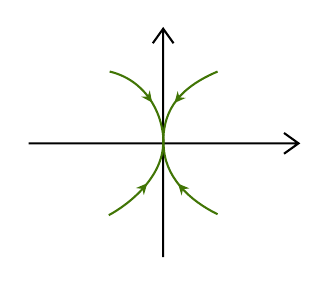
\begin{tikzpicture}[x=0.75pt,y=0.75pt,yscale=-1,xscale=1]
		%uncomment if require: \path (0,300); %set diagram left start at 0, and has height of 300
		
		%Shape: Axis 2D [id:dp9380995091348139] 
		\draw  (130,135.23) -- (260,135.23)(194.78,80) -- (194.78,190) (253,130.23) -- (260,135.23) -- (253,140.23) (189.78,87) -- (194.78,80) -- (199.78,87)  ;
		%Curve Lines [id:da7464742185837894] 
		\draw [color={rgb, 255:red, 65; green, 117; blue, 5 }  ,draw opacity=1 ]   (194.78,135.23) .. controls (194.78,122.17) and (199.33,109.79) .. (221,100.63) ;
		\draw [shift={(200.24,115.76)}, rotate = 310.45] [fill={rgb, 255:red, 65; green, 117; blue, 5 }  ,fill opacity=1 ][line width=0.08]  [draw opacity=0] (5.36,-2.57) -- (0,0) -- (5.36,2.57) -- (3.56,0) -- cycle    ;
		%Curve Lines [id:da3247666901842563] 
		\draw [color={rgb, 255:red, 65; green, 117; blue, 5 }  ,draw opacity=1 ]   (168.57,169.83) .. controls (178.33,164.67) and (194.57,151.5) .. (194.78,135.23) ;
		\draw [shift={(187.11,154.49)}, rotate = 131.69] [fill={rgb, 255:red, 65; green, 117; blue, 5 }  ,fill opacity=1 ][line width=0.08]  [draw opacity=0] (5.36,-2.57) -- (0,0) -- (5.36,2.57) -- (3.56,0) -- cycle    ;
		%Curve Lines [id:da34070001099076586] 
		\draw [color={rgb, 255:red, 65; green, 117; blue, 5 }  ,draw opacity=1 ]   (221,169.38) .. controls (207.78,162.96) and (194.78,151.27) .. (195,135) ;
		\draw [shift={(201.96,154.66)}, rotate = 47.94] [fill={rgb, 255:red, 65; green, 117; blue, 5 }  ,fill opacity=1 ][line width=0.08]  [draw opacity=0] (5.36,-2.57) -- (0,0) -- (5.36,2.57) -- (3.56,0) -- cycle    ;
		%Curve Lines [id:da12862086047130106] 
		\draw [color={rgb, 255:red, 65; green, 117; blue, 5 }  ,draw opacity=1 ]   (195,135) .. controls (194.57,118.96) and (185.25,104.52) .. (169,100.63) ;
		\draw [shift={(189.43,115.52)}, rotate = 233.71] [fill={rgb, 255:red, 65; green, 117; blue, 5 }  ,fill opacity=1 ][line width=0.08]  [draw opacity=0] (5.36,-2.57) -- (0,0) -- (5.36,2.57) -- (3.56,0) -- cycle    ;
		
		
		
		
	\end{tikzpicture}
	
	
\end{figure}

Thus the stable sets of the invariant sets of this system will be
\[ W^s(S_1)=\R^2,\qquad W^s(S_2)=\R^2, \qquad W^s(S_3)=\R^2. \]

With a similar logic, we can define the \textbf{unstable set $ W^u(S)$} of in invariant set, which is the set of all states whose orbits approach $S$ \emph{backward} in time.

\begin{corbox}
	The stable, and unstable sets of an invariant set, are invariant sets themselves.
\end{corbox}
\begin{proof}
	Here we proof the statement for the unstable set only, however, the proof logic for both of them is similar. We proceed with the proof by contradiction. Assume that $W^s(S)$ is not a invariant set. This means that 
	\[ \exists x_0\in W^s(S),\ \exists t^*\in\R, \st\ \phi^{t^*} x_0 = z_0  \notin W^s(S).  \]
	So $\lim_{t\to\infty} d(\phi^t z_0, S) \neq 0$. On the other hand, because of  $\phi^{s+t}x_0 = \phi^s (\phi^t x_0)$ we have
	\begin{align*}
		\phi^{t^*}x_0 = z_0 \ \Leftrightarrow\ \phi^{t-t^*}(\phi^{t^*}x_0)= \phi^{t-t^*} z_0\ \Leftrightarrow\ \phi^t x = \phi^{t-t^*} z_0,
	\end{align*}
	which implies that the distance between $\phi^{t-t^*}z_0$ and the set $S$ goes to zero, which contradicts our assumption. So we conclude that the stable set of an invariant set, is an invariant set itself.

\end{proof}

